%!TEX root = ../thesis.tex

\centering
  \begin{subfigure}[b]{0.98\textwidth}
    \centering
      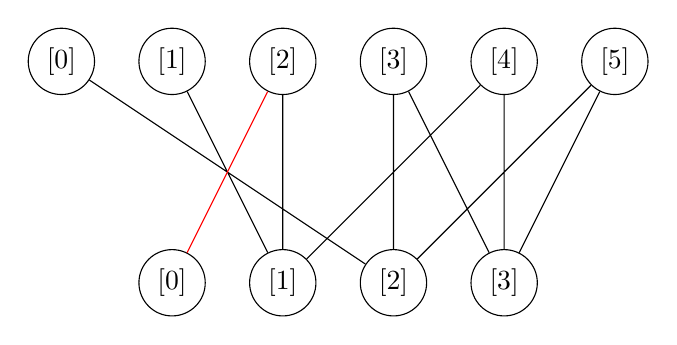
\begin{tikzpicture}
        {\tikzstyle{every node}=[circle, draw]
          \foreach \i in {0, ..., 5}
          {
            \node (s\i) at (\i*40pt, 80pt) {\species[\i]};
          }

          \foreach \j in {0, ..., 3}
          {
            \node (c\j) at (\j*40pt+40pt, 0) {\character[\j]};
          }
        }

        \draw
          (c3) -- (s3)
          (c3) -- (s4)
          (c3) -- (s5)
          (c1) -- (s1)
          (c1) -- (s2)
          (c1) -- (s4)
          (c2) -- (s0)
          (c2) -- (s3)
          (c2) -- (s5);

        \draw[red]
          (c0) -- (s2);
      \end{tikzpicture}

    \caption{Maximal reducible graph \gm{}}
    \label{figure:4:a}
  \end{subfigure}

  \bigskip

  \begin{subfigure}[b]{0.98\textwidth}
    \centering
      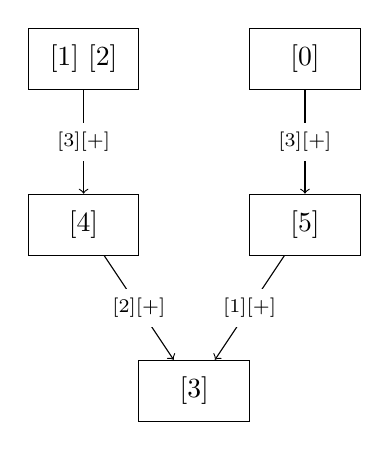
\begin{tikzpicture}
        {\tikzstyle{every node}=[rectangle, draw, minimum width=40pt, minimum height=22pt]
          \node (s1) at (0pt,  120pt) {\species[1] \species[2]};
          \node (s0) at (80pt, 120pt) {\species[0]};
          \node (s4) at (0pt,   60pt) {\species[4]};
          \node (s5) at (80pt,  60pt) {\species[5]};
          \node (s3) at (40pt,   0pt) {\species[3]};
        }

        {\tikzstyle{every node}=[fill=white, font=\scriptsize]
          \draw
            (s0) edge[->] node{\character[3][+]} (s5)
            (s1) edge[->] node{\character[3][+]} (s4)
            (s4) edge[->] node{\character[2][+]} (s3)
            (s5) edge[->] node{\character[1][+]} (s3);
        }
      \end{tikzpicture}

    \caption{Hasse diagram \hasse{} for \gm{}}
    \label{figure:4:b}
  \end{subfigure}
